% =====================================================================
% Reporte: Visual Servoing para destapado de botellas con xArm6
% Formato: IEEE Conference (IEEEtran). Listo para Overleaf.
% =====================================================================
\documentclass[conference]{IEEEtran}
\IEEEoverridecommandlockouts

\usepackage[spanish,es-tabla]{babel}
\usepackage[utf8]{inputenc}
\usepackage[T1]{fontenc}
\usepackage{cite}
\usepackage{amsmath,amssymb,amsfonts}
\usepackage{algorithmic}
\usepackage{graphicx}
\graphicspath{{Graficas/}}
\usepackage{textcomp}
\usepackage{xcolor}
\usepackage{url}
\usepackage{hyperref}
\usepackage{booktabs}
\usepackage{listings}
\usepackage{siunitx}

\hypersetup{
  colorlinks=true,
  linkcolor=blue!60!black,
  urlcolor=blue!60!black,
  citecolor=blue!60!black,
}

\lstset{
  basicstyle=\ttfamily\footnotesize,
  breaklines=true,
  columns=fullflexible,
  frame=single,
  keepspaces=true,
}

\def\BibTeX{{\rm B\kern-.05em{\sc i\kern-.025em b}\kern-.08em
    T\kern-.1667em\lower.7ex\hbox{E}\kern-.125emX}}

\begin{document}

\title{Visual Servoing\\[2pt]
\large Servovisi\'on con MPC sobre xArm6 para el destapado aut\'onomo de
botellas usando un descorchador de pared y dos c\'amaras ZED}

\author{
\IEEEauthorblockN{Gerardo Fregoso Jim\'enez}
\IEEEauthorblockA{IRS\,|\,A00838645}
\and
\IEEEauthorblockN{Luis Fernando Ruiz Neria}
\IEEEauthorblockA{IRS\,|\,A00839528}
\and
\IEEEauthorblockN{Jos\'e Ra\'ul Arredondo L\'opez}
\IEEEauthorblockA{IRS\,|\,A01742153}
\and
\IEEEauthorblockN{Daniel Eduardo Hinojosa Alvarado}
\IEEEauthorblockA{IRS\,|\,A00838156}
}

\maketitle

\begin{center}
\vspace{-0.5em}
\textbf{Instituto Tecnol\'ogico y de Estudios Superiores de Monterrey}\\
Campus Monterrey\\[2pt]
\textbf{TE3002B} -- Implementaci\'on de Rob\'otica Inteligente\\[2pt]
Fecha de entrega: 24 de marzo de 2026\\[6pt]
\end{center}

\begin{abstract}
Se presenta un sistema de manipulaci\'on aut\'onoma que utiliza un brazo
rob\'otico UFactory xArm6 equipado con un gripper personalizado y dos
c\'amaras estereosc\'opicas StereoLabs ZED para localizar, sujetar,
transportar y destapar una botella mediante un descorchador montado en
una pared. La detecci\'on visual se realiza con AprilTags
(\texttt{tag36h11}) y la aproximaci\'on al objeto se gobierna mediante
un controlador predictivo basado en modelo (MPC) de 6~grados de
libertad que opera en el espacio de tarea y publica twists Cartesianos
a MoveIt~Servo. Todo el sistema corre en una Jetson Orin AGX, sobre
ROS\,2~Humble con MoveIt y Cyclone~DDS, integrado al stack de
manipulaci\'on \emph{home2} del equipo RoBorregos. El pipeline completo
consta de siete etapas (pre-grasp, MPC, lift-up, drop, alineaci\'on en
imagen, aproximaci\'on, twist de destape) ejecutadas por un
orquestador en Python. Las pruebas experimentales --- documentadas en
los videos adjuntos en este directorio --- muestran que el robot
consigue agarrar, posicionar y destapar la botella de forma repetible.
\end{abstract}

\begin{IEEEkeywords}
servovisi\'on, MPC, AprilTag, xArm6, ZED, ROS\,2, MoveIt, manipulaci\'on.
\end{IEEEkeywords}

% =====================================================================
\section{Introducci\'on}
% =====================================================================

El destapado de una botella mediante un descorchador fijo en pared es
una tarea que combina manipulaci\'on de precisi\'on, alineaci\'on
visual y restricciones geom\'etricas: el robot debe (i) localizar la
botella sobre la mesa, (ii) sujetarla con un agarre repetible,
(iii) llevarla hasta el descorchador y (iv) introducir la tapa en el
mecanismo manteniendo el eje del cuello alineado con la mordaza del
descorchador. Cualquier error angular o lateral mayor a unos pocos
mil\'imetros provoca que la tapa no quede bien enganchada.

Para resolver el problema se desarroll\'o un sistema completo de
servovisi\'on que combina dos lazos cerrados visuales: el primero, en
configuraci\'on \emph{eye-in-hand} con una c\'amara ZED montada en el
gripper, lleva al brazo desde una pose de pre-agarre hasta el agarre
de la botella usando un controlador MPC; el segundo, en
configuraci\'on \emph{eye-to-hand} con una segunda ZED fija que observa
la zona del descorchador, alinea la botella en p\'ixeles y la conduce
hasta la posici\'on de destape mediante una aproximaci\'on basada en
el tama\'no aparente de los AprilTags.

El sistema se desarrolla como extensi\'on del stack
\emph{home2}~\cite{roborregos-home2} de RoBorregos --- el cual provee
la configuraci\'on de MoveIt para el xArm6, el contenedor de
manipulaci\'on y los lanzadores de ROS\,2 --- y se integra al
repositorio del equipo (m\'odulo \texttt{Control\_Module/Visual\_%
Servoing\_Project}). Los aportes principales de este trabajo son:

\begin{itemize}
  \item Procedimiento de calibraci\'on \emph{hand--eye} para
        determinar la transformaci\'on est\'atica
        \texttt{gripper}$\rightarrow$\texttt{zed} y persistirla en el
        URDF.
  \item Controlador MPC de 6~DOF con restricciones de caja sobre la
        velocidad Cartesiana, linealizado en cada ciclo, que conduce
        el gripper hasta una pose demostrada relativa al AprilTag de
        la botella.
  \item Dos m\'odulos de alineaci\'on en espacio de imagen usando una
        segunda c\'amara fija, uno para centrar la tapa y otro para
        aproximarse en el eje X de la base hasta dos tama\'nos
        objetivo de AprilTag (\emph{far} y \emph{near}).
  \item Orquestador de pipeline de 7~etapas que gestiona MoveIt y
        Servo de forma coordinada, evitando los conflictos del
        controlador de trayectoria compartido.
\end{itemize}

El c\'odigo, los lanzadores, las plantillas de AprilTag y la presente
documentaci\'on est\'an disponibles en el directorio
\texttt{Control\_Module/Visual\_Servoing\_Project} del repositorio del
equipo.

% =====================================================================
\section{Sistema y Materiales}
% =====================================================================

\subsection{Hardware}

\begin{itemize}
  \item \textbf{Brazo}: UFactory xArm6 (6~DOF), montado en mesa de
        trabajo. Comunicaci\'on por Ethernet.
  \item \textbf{Gripper}: efector final paralelo personalizado del
        equipo, controlado por una salida digital del controlador del
        xArm (\texttt{/xarm/set\_tgpio\_digital}).
  \item \textbf{C\'amaras}: dos StereoLabs ZED.
        \begin{itemize}
          \item \emph{ZED \#1 (eye-in-hand)}: atornillada al cuerpo
                del gripper. Provee la pose del AprilTag de la botella
                relativa al efector y se usa para el lazo MPC.
          \item \emph{ZED \#2 (eye-to-hand)}: fija frente al
                descorchador. Provee la imagen rectificada con la que
                se centra la tapa y se ejecuta la aproximaci\'on por
                tama\'no de tag.
        \end{itemize}
  \item \textbf{C\'omputo}: NVIDIA Jetson Orin AGX
        (\texttt{orin@192.168.31.10}), ejecutando todo dentro de un
        contenedor Docker basado en L4T.
  \item \textbf{AprilTags}: familia \texttt{tag36h11}. Tag \texttt{0}
        para calibraci\'on (\SI{133}{\milli\meter} de lado), tag
        \texttt{13} sobre la tapa de la botella, tags \texttt{1}
        (NEAR) y \texttt{2} (FAR) sobre el descorchador.
  \item \textbf{Descorchador}: dispositivo comercial de pared, fijo
        durante todo el experimento.
\end{itemize}

\subsection{Software}

El sistema corre sobre ROS\,2~Humble con MoveIt2, MoveIt~Servo, el
driver oficial del xArm, \texttt{apriltag\_ros}~3.3.0 y Cyclone~DDS
como middleware. Se reutiliza el stack \texttt{home2} de
RoBorregos~\cite{roborregos-home2}: el lanzador
\texttt{frida\_moveit\_config.launch.py} ya integra MoveIt + driver
del xArm, y el contenedor de manipulaci\'on (\texttt{run.sh
manipulation}) provee las dependencias congeladas. El c\'odigo
nuevo --- \emph{collectsamples}, \emph{solve\_handeye}, \emph{mpc\_vs\_pick},
\emph{align\_*} y \emph{pick\_pipeline} --- vive en
\texttt{/home/orin/dev/nav/visual\_servoing/} en el host y se monta
dentro del contenedor como \texttt{/workspace/src/visual\_servoing/}.

\subsection{Frames y convenciones}

Se utilizan los siguientes frames principales:

\begin{itemize}
  \item \texttt{link\_base}: ra\'iz del xArm6 (base del brazo).
  \item \texttt{gripper}: link al que est\'a soldado el efector y
        relativo al cual se calibra la ZED~\#1.
  \item \texttt{zed\_left\_camera\_optical\_frame}: \'optica izquierda
        de la ZED~\#1, donde \texttt{apriltag\_ros} publica las
        detecciones.
  \item \texttt{tag36h11\_0}, \texttt{tag36h11\_13}, etc.: frames
        publicados por el detector para cada tag visible.
\end{itemize}

% =====================================================================
\section{Calibraci\'on \emph{hand--eye}}
% =====================================================================

Para que la ZED~\#1 sea \'util en el lazo MPC, el URDF debe reflejar
con precisi\'on c\'omo est\'a montada respecto al \texttt{gripper}.
Esto se resuelve con una calibraci\'on \emph{hand--eye} en variante
\emph{eye-in-hand}: con la c\'amara fija al efector y un AprilTag
est\'atico en la escena, se busca la transformaci\'on
$T_{gripper}^{zed}$ que satisface, para un conjunto de capturas
$\{i\}$:
\begin{equation}
T_{base}^{gripper_i} \cdot T_{gripper}^{zed} \cdot
T_{zed}^{tag_i} = T_{base}^{tag} = \text{constante.}
\label{eq:handeye}
\end{equation}

\subsection{Pipeline de calibraci\'on}

Se implementaron tres scripts en
\texttt{tools/calibration/}:

\begin{itemize}
  \item \texttt{collect\_samples.py}: con el brazo en \emph{freedrive},
        captura por cada pose el par
        $(T_{base}^{gripper_i},\, T_{zed}^{tag_i})$ usando tf2.
        Se exportan 12--20 muestras con suficiente variedad en
        rotaci\'on (al menos $15$--$30^\circ$ entre muestras
        consecutivas) y traslaci\'on.
  \item \texttt{solve\_handeye.py}: resuelve
        \eqref{eq:handeye} usando los cinco m\'etodos disponibles en
        \texttt{cv2.calibrateHandEye} (TSAI, PARK, HORAUD, ANDREFF,
        DANIILIDIS) y reporta RMS residual de la posici\'on del tag
        reconstruida en \texttt{link\_base}.
  \item \texttt{apply\_to\_urdf.py}: edita el origen del
        \texttt{<joint name="ZED">} en \texttt{gripper.xacro} dentro
        de \texttt{frida\_description} y deja un respaldo
        \texttt{.bak} antes de sobrescribir.
\end{itemize}

\subsection{Criterio de \'exito}

Se considera la calibraci\'on aceptable cuando los cinco m\'etodos
coinciden en pocos mil\'imetros y pocos grados, y el RMS residual es
inferior a \SI{10}{\milli\meter}. Tras aplicar el resultado al URDF
y reconstruir \texttt{frida\_description}, la nube de puntos de la
ZED se sobrepone correctamente a la geometr\'ia simulada en RViz.

% =====================================================================
\section{Control predictivo (MPC) para el agarre}
% =====================================================================

La etapa de agarre utiliza la ZED~\#1 (eye-in-hand) para conducir el
gripper hasta una pose demostrada relativa al AprilTag de la botella.

\subsection{Captura de la pose objetivo}

El script \texttt{record\_goal\_pose.py} se ejecuta una sola vez con
el brazo posicionado manualmente en la \emph{configuraci\'on de cierre
de pinza}: pega un snapshot de
$T_{gripper}^{tag}$ a un YAML
(\texttt{goal\_pose.yaml}) que servir\'a de referencia constante al
controlador.

\subsection{Formulaci\'on del MPC}

Definimos el estado de error como
$\mathbf{e}\in\mathbb{R}^6 = (\Delta\mathbf{p}, \Delta\mathbf{r})$,
donde $\Delta\mathbf{p}$ es el error de traslaci\'on y
$\Delta\mathbf{r}$ es la representaci\'on eje--\'angulo del error
rotacional entre la pose actual y la deseada, ambos expresados en el
marco \texttt{gripper}. El control es el twist Cartesiano del gripper:
$\mathbf{u}\in\mathbb{R}^6 = (\mathbf{v}, \boldsymbol{\omega})$.

\paragraph*{Din\'amica linealizada} Tomando un paso de integraci\'on
$\Delta t$ y re-linealizando alrededor del estado actual cada ciclo
de control:
\begin{equation}
\mathbf{e}_{k+1} = \mathbf{e}_k + \Delta t \cdot M \cdot \mathbf{u}_k,
\quad
M = \begin{bmatrix} -I_3 & [\mathbf{p}]_\times \\ 0 & -I_3 \end{bmatrix},
\label{eq:dynamics}
\end{equation}
donde $[\mathbf{p}]_\times$ es la matriz antisim\'etrica asociada a
la traslaci\'on actual del tag en el frame del gripper. Aunque el
modelo es lineal en cada ciclo, la re-linealizaci\'on a cada paso
permite seguir grandes rotaciones de forma robusta.

\paragraph*{Funci\'on de costo}
\begin{equation}
J = \sum_{k=1}^{N} \mathbf{e}_k^\top Q\, \mathbf{e}_k
  + \sum_{k=0}^{N-1} \mathbf{u}_k^\top R\, \mathbf{u}_k
  + \mathbf{e}_N^\top Q_f\, \mathbf{e}_N,
\label{eq:cost}
\end{equation}
con $Q_f = \alpha\,Q$ (por defecto $\alpha=10$) para penalizar
fuertemente el error terminal.

\paragraph*{Restricciones} Caja sobre cada componente del control:
\begin{equation}
|v_i| \le v_{\max},\qquad |\omega_i| \le \omega_{\max}.
\end{equation}

\paragraph*{Solver} Se concatenan los controles en
$\mathbf{z} = [\mathbf{u}_0; \dots; \mathbf{u}_{N-1}]\in\mathbb{R}^{6N}$
y se resuelve con L-BFGS-B de SciPy. La soluci\'on del ciclo anterior
se reutiliza desplazada un paso (\emph{warm-start}), patr\'on est\'andar
en MPC de horizonte recedente. Se aplica solo $\mathbf{u}_0$ y se
re-observa.

\subsection{Seguridad}

\begin{itemize}
  \item El controlador env\'ia twist cero si el tag se pierde por m\'as
        de \SI{1}{\second}.
  \item L\'imite por defecto de \SI{0.03}{\meter\per\second} y
        \SI{0.3}{\radian\per\second} al iniciar; se suben tras
        verificar comportamiento.
  \item \texttt{Ctrl+C} publica un twist cero al salir.
  \item \texttt{/servo\_node/stop\_servo} act\'ua como interruptor de
        emergencia.
  \item Antes de cada cambio relevante se ejecuta con
        \texttt{--dry-run} (sin publicar twists) para validar signos
        y direcciones.
\end{itemize}

Cuando $\|\Delta\mathbf{p}\| < t_\text{tol}$ y
$\|\Delta\mathbf{r}\| < r_\text{tol}$, el MPC dispara el cierre del
gripper v\'ia \texttt{/xarm/set\_tgpio\_digital} y termina.

% =====================================================================
\section{Alineaci\'on en espacio de imagen con la segunda c\'amara}
% =====================================================================

Tras el agarre, la botella se transporta a la zona del descorchador.
La precisi\'on requerida para introducir la tapa supera lo que ofrece
una sola planificaci\'on en espacio articular, por lo que se utiliza
una segunda ZED, fija, que observa el rea del descorchador con un
\'angulo de vista \emph{cenital y lateral}. Esta c\'amara alimenta dos
m\'odulos en \texttt{tools/align/}.

\subsection{\texttt{align\_top\_tag.py} -- centrar la tapa}

Detecta el AprilTag \texttt{id 13} pegado en la tapa de la botella y
publica un twist Cartesiano $(v_x, v_y)$ a
\texttt{/servo\_node/delta\_twist\_cmds} proporcional al error en
p\'ixeles entre el centroide del tag y un \emph{target} guardado en
\texttt{align\_target.yaml}. El target se captura previamente con
\texttt{--save-target} desde una pose donde la tapa qued\'o
visualmente alineada con la boca del descorchador.

Par\'ametros por defecto:
\begin{itemize}
  \item ganancia $K_p = 0.001$ (m/s por p\'ixel),
  \item velocidad m\'axima \SI{0.2}{\meter\per\second},
  \item tolerancia de aceptaci\'on \SI{25}{\pixel}.
\end{itemize}
Los flags \texttt{--invert-x} y \texttt{--invert-y} corrigen el signo
seg\'un la orientaci\'on real de la c\'amara fija.

\subsection{\texttt{align\_approach\_tag.py} -- aproximaci\'on por
            tama\'no de tag}

Una vez centrada la tapa, el brazo avanza en el eje X de la base hasta
quedar a la distancia exacta del descorchador. Se evita usar
profundidad directa de la ZED (ruidosa en distancias cortas) y, en su
lugar, se utiliza el \emph{tama\'no aparente en p\'ixeles} de un
AprilTag fijo sobre el descorchador.

Para tolerar el rango de operaci\'on completo (desde varios cm hasta
contacto) se usan dos tags:
\begin{itemize}
  \item Tag \texttt{2} (\emph{FAR}): visible desde lejos, m\'as
        grande f\'isicamente, gobierna la primera fase a velocidad
        normal (\texttt{--max-speed}).
  \item Tag \texttt{1} (\emph{NEAR}): m\'as peque\'no y a menor
        distancia; el controlador conmuta a este tag tan pronto como
        sea detectable de manera estable, y limita la velocidad
        (\texttt{--near-max-speed}) para arribar suave al target.
\end{itemize}
Adicionalmente se controla un peque\'no offset en Z mediante el
componente vertical del tag NEAR (\texttt{--gain-z},
\texttt{--max-speed-z}, \texttt{--tol-v-px}) para llegar
simult\'aneamente en X y en Z.

Los targets de tama\'no de tag se capturan con
\texttt{--save-far} y \texttt{--save-near} desde la pose donde el
mecanismo del descorchador ya enganch\'o correctamente la tapa, y se
combinan en \texttt{approach\_target.yaml}.

% =====================================================================
\section{Pipeline integral de 7 etapas}
% =====================================================================

El orquestador \texttt{pick\_pipeline.py} encadena los m\'odulos
anteriores en una sola secuencia.

\begin{figure*}[!t]
\centering
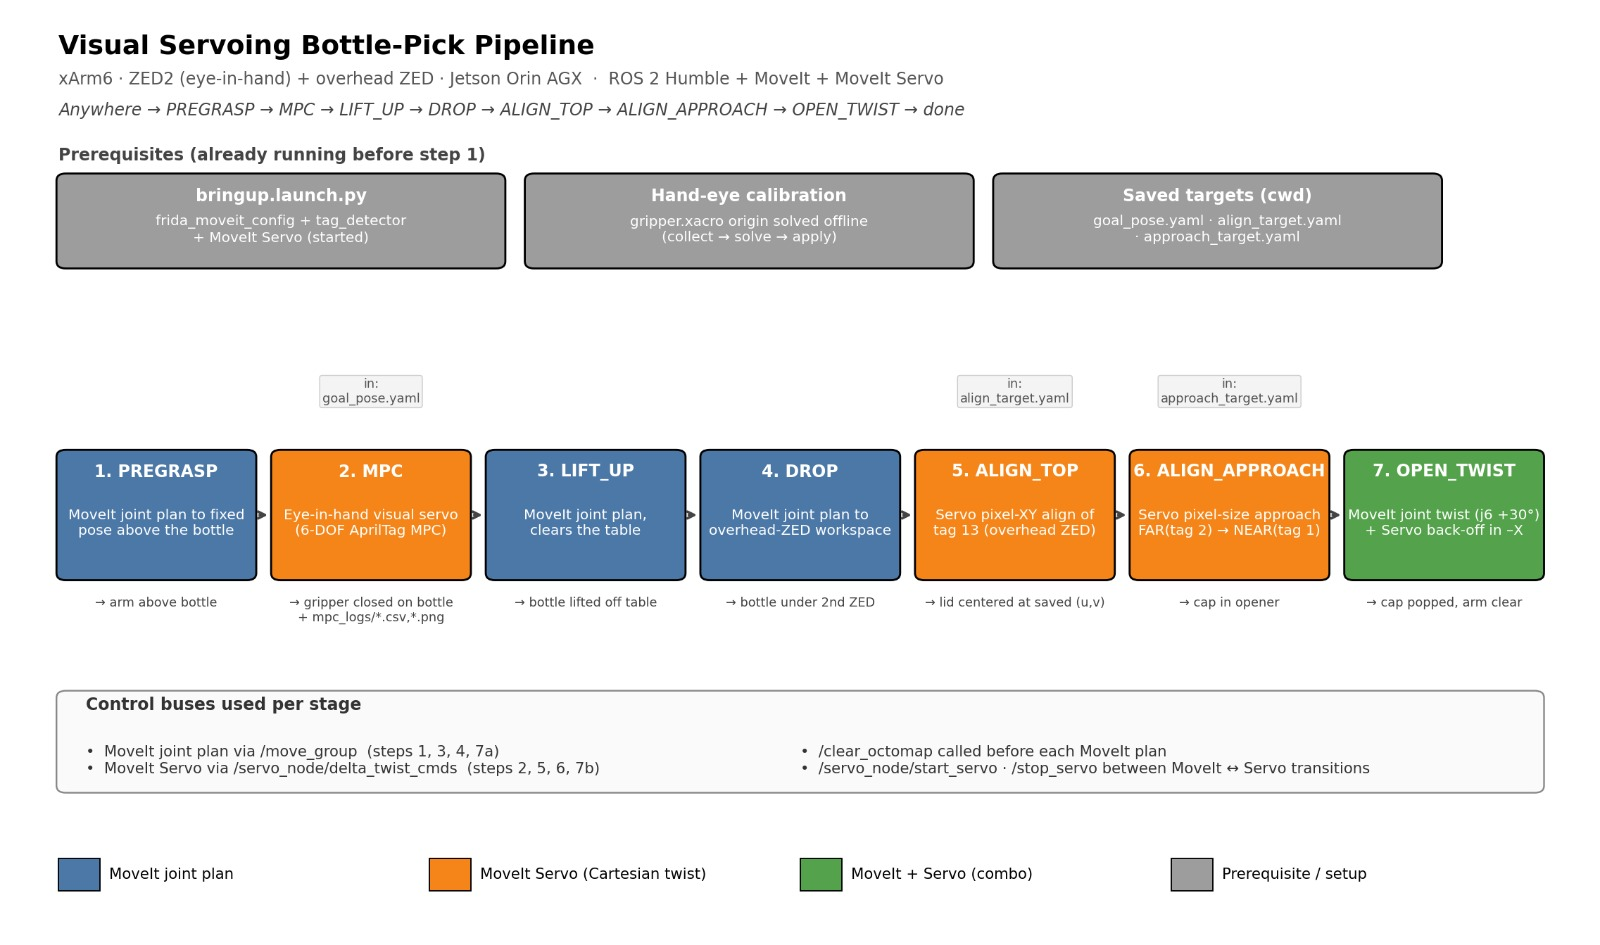
\includegraphics[width=0.95\textwidth]{pipeline.jpeg}
\caption{Diagrama del pipeline completo de destape de botellas. La
parte superior agrupa los \emph{prerequisitos} que deben estar
corriendo antes de la primera etapa: \texttt{bringup.launch.py}
(MoveIt + Servo + detector de tags), la calibraci\'on \emph{hand--eye}
ya aplicada al URDF y los tres YAML de configuraci\'on guardados en el
directorio de trabajo (\texttt{goal\_pose.yaml},
\texttt{align\_target.yaml} y \texttt{approach\_target.yaml}). La
fila central muestra las siete etapas en orden, codificadas por color
seg\'un el bus de control: azul para metas articulares de MoveIt,
naranja para servovisi\'on con MoveIt~Servo y verde para la etapa
combinada (twist articular + back-off Cartesiano). Debajo de cada
caja se indica el resultado f\'isico esperado (\textit{p.\,ej.}
\emph{bottle lifted off table} o \emph{cap in opener}). El recuadro
inferior resume las dos rutas de control utilizadas y la coreograf\'ia
\texttt{start\_servo}/\texttt{stop\_servo} necesaria entre transiciones
MoveIt$\leftrightarrow$Servo, junto con el \texttt{/clear\_octomap}
previo a cada planificaci\'on.}
\label{fig:pipeline}
\end{figure*}

La Fig.~\ref{fig:pipeline} resume gr\'aficamente las siete etapas y los
prerequisitos que el sistema debe tener activos antes de comenzar.

\begin{table}[h]
\centering
\caption{Etapas del pipeline de destape.}
\label{tab:pipeline}
\begin{tabular}{cll}
\toprule
\# & Etapa & Lazo de control \\
\midrule
1 & PREGRASP        & MoveIt -- meta articular \\
2 & MPC             & Servovisi\'on eye-in-hand \\
3 & LIFT\_UP        & MoveIt -- meta articular \\
4 & DROP            & MoveIt -- meta articular \\
5 & ALIGN\_TOP      & P\'ixeles -- ZED~\#2 \\
6 & ALIGN\_APPROACH & Tama\'no de tag -- ZED~\#2 \\
7 & OPEN\_TWIST     & MoveIt + Servo (back-off) \\
\bottomrule
\end{tabular}
\end{table}

\subsection{Detalle de etapas}

\begin{enumerate}
  \item \textbf{PREGRASP}: meta articular fija ($\mathbf{q}_\text{pg}$)
        que coloca el brazo arriba de la mesa con la botella en
        campo visual de la ZED~\#1. Se planea con MoveIt (las metas
        articulares siempre tienen IK v\'alida, lo cual evita
        fracasos de OMPL en metas Cartesianas).
  \item \textbf{MPC}: subproceso \texttt{mpc\_vs\_pick.py}.
        Conduce el gripper hasta la pose demostrada,
        dispara el cierre y termina.
  \item \textbf{LIFT\_UP}: meta articular ligeramente elevada
        (5--10~cm sobre PREGRASP) para liberar la botella del nivel
        de la mesa antes de moverse lateralmente.
  \item \textbf{DROP}: meta articular que lleva la botella al \'area
        de trabajo donde la ZED~\#2 ve la tapa.
  \item \textbf{ALIGN\_TOP}: subproceso \texttt{align\_top\_tag.py}.
        Centra la tapa al p\'ixel guardado.
  \item \textbf{ALIGN\_APPROACH}: subproceso
        \texttt{align\_approach\_tag.py}. Aproxima el conjunto
        botella+tapa hasta el descorchador con la conmutaci\'on
        FAR$\rightarrow$NEAR.
  \item \textbf{OPEN\_TWIST}: rotaci\'on de \SI{+30}{\degree} del
        \texttt{joint6} (por defecto, ajustable) v\'ia meta articular
        de MoveIt, seguido de un \emph{back-off} Cartesiano de
        \SI{5}{\centi\meter} en el eje X de la base servido por
        Servo, que retira la botella del mecanismo dejando la tapa
        atrapada en el descorchador.
\end{enumerate}

\subsection{Gesti\'on de Servo vs.\ MoveIt}

MoveIt~Servo y el planificador de MoveIt comparten el mismo
controlador de trayectoria (\texttt{/xarm6\_traj\_controller}). Si
Servo lo mantiene reclamado, una planificaci\'on de MoveIt falla
silenciosamente. El pipeline maneja esto expl\'icitamente: detiene
Servo con \texttt{/servo\_node/stop\_servo} antes de las etapas
basadas en MoveIt (LIFT\_UP, DROP, OPEN\_TWIST) y lo reinicia con
\texttt{/servo\_node/start\_servo} antes de cada etapa basada en
Servo (ALIGN\_TOP, ALIGN\_APPROACH, back-off del OPEN\_TWIST). Antes
de cada planificaci\'on se limpia el octomap.

% =====================================================================
\section{Resultados}
% =====================================================================

El sistema completo fue evaluado sobre la celda real con el
descorchador montado en la pared del laboratorio. El brazo parte
desde una pose arbitraria, ejecuta las siete etapas y deja la tapa
removida en el descorchador. Las pruebas se documentan en los videos
de demostraci\'on adjuntos en este mismo directorio
(\texttt{Control\_Module/Visual\_Servoing\_Project/}).

\begin{table}[h]
\centering
\caption{Resumen del estado de cada componente.}
\label{tab:status}
\begin{tabular}{ll}
\toprule
Componente & Estado \\
\midrule
Stack de manipulaci\'on (MoveIt + xArm) & Operativo \\
ZED + tf publicando & Operativo \\
\texttt{apriltag\_ros} 3.3.0 en contenedor & Operativo \\
Calibraci\'on \emph{hand--eye} & Aplicada al URDF \\
MPC eye-in-hand para agarre & Operativo \\
ALIGN\_TOP (ZED~\#2) & Operativo \\
ALIGN\_APPROACH (FAR$\rightarrow$NEAR) & Operativo \\
Pipeline de 7 etapas end-to-end & Operativo \\
\bottomrule
\end{tabular}
\end{table}

\subsection{Desempe\~no experimental del MPC}

Para evaluar cuantitativamente la etapa de servovisi\'on se registr\'o
una corrida representativa del MPC durante el agarre
(\texttt{mpc\_20260515\_013427.csv}, 204 ticks de control,
\textbf{0~p\'erdidas} de tag en toda la corrida). De este registro
se generaron las cuatro gr\'aficas siguientes.

\subsubsection{Convergencia global del error}

\begin{figure}[!t]
\centering
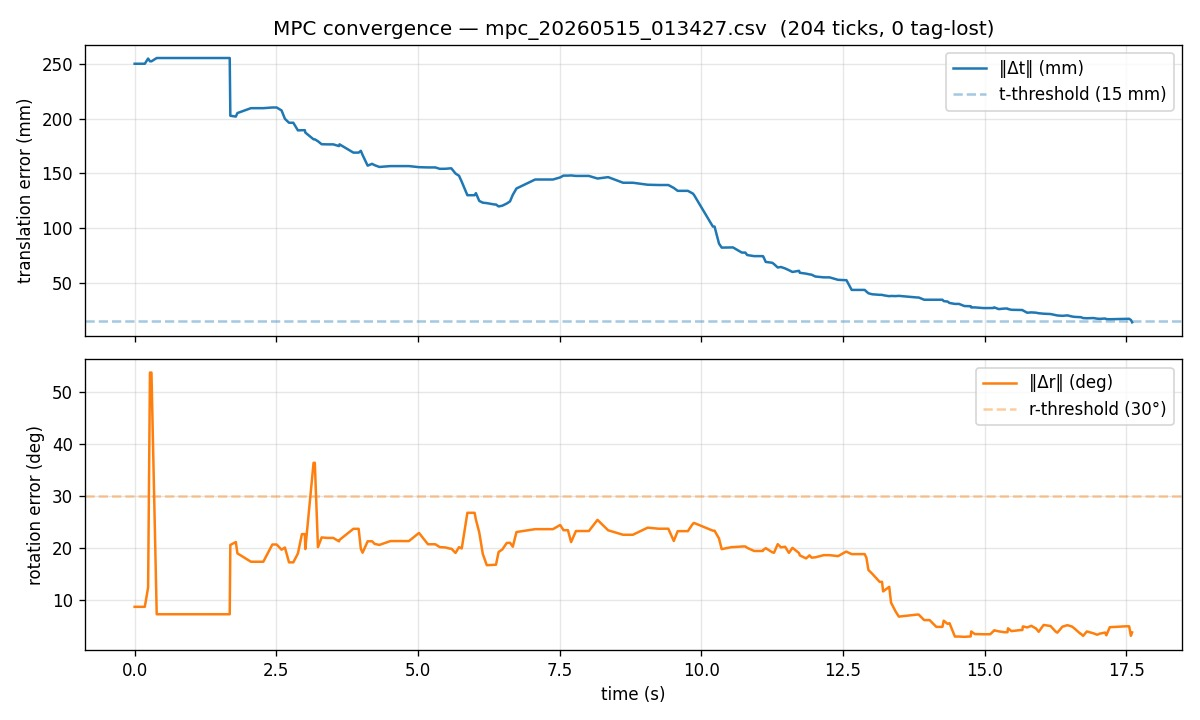
\includegraphics[width=\columnwidth]{mpc_convergence.jpeg}
\caption{Convergencia del error tag-en-gripper durante una corrida
completa del MPC. Arriba: norma del error de traslaci\'on
$\lVert\Delta\mathbf{t}\rVert$ en mm; abajo: norma del error de
rotaci\'on $\lVert\Delta\mathbf{r}\rVert$ en grados. Las l\'ineas
punteadas marcan los umbrales de aceptaci\'on
(\SI{15}{\milli\meter} y \SI{30}{\degree}) a partir de los cuales el
MPC declara la pose alcanzada y dispara el cierre del gripper.}
\label{fig:mpc-convergence}
\end{figure}

La Fig.~\ref{fig:mpc-convergence} muestra c\'omo el error de
traslaci\'on parte de $\sim$\SI{255}{\milli\meter} y desciende
mon\'otonamente hasta cruzar el umbral de \SI{15}{\milli\meter} cerca
de $t\!\approx\!\SI{17}{\second}$, sin oscilaciones ni rebotes
visibles. El error de rotaci\'on se mantiene durante la primera mitad
de la corrida en torno a \SI{20}{\degree} --- por debajo del umbral
de \SI{30}{\degree} pero sin caer ---, lo cual es consistente con un
MPC que prioriza traer la traslaci\'on al objetivo (matriz $Q$ con
mayor peso en posici\'on) y solo refina la orientaci\'on en la fase
final, donde efectivamente colapsa hasta unos pocos grados. Los dos
escalones de la traslaci\'on alrededor de $t\!\approx\!\SI{1.5}{\second}$
y $t\!\approx\!\SI{10}{\second}$ corresponden a momentos en que el
detector AprilTag publica una pose ligeramente reproyectada al
recuperar nitidez en la imagen.

\subsubsection{Descomposici\'on del error por eje}

\begin{figure}[!t]
\centering
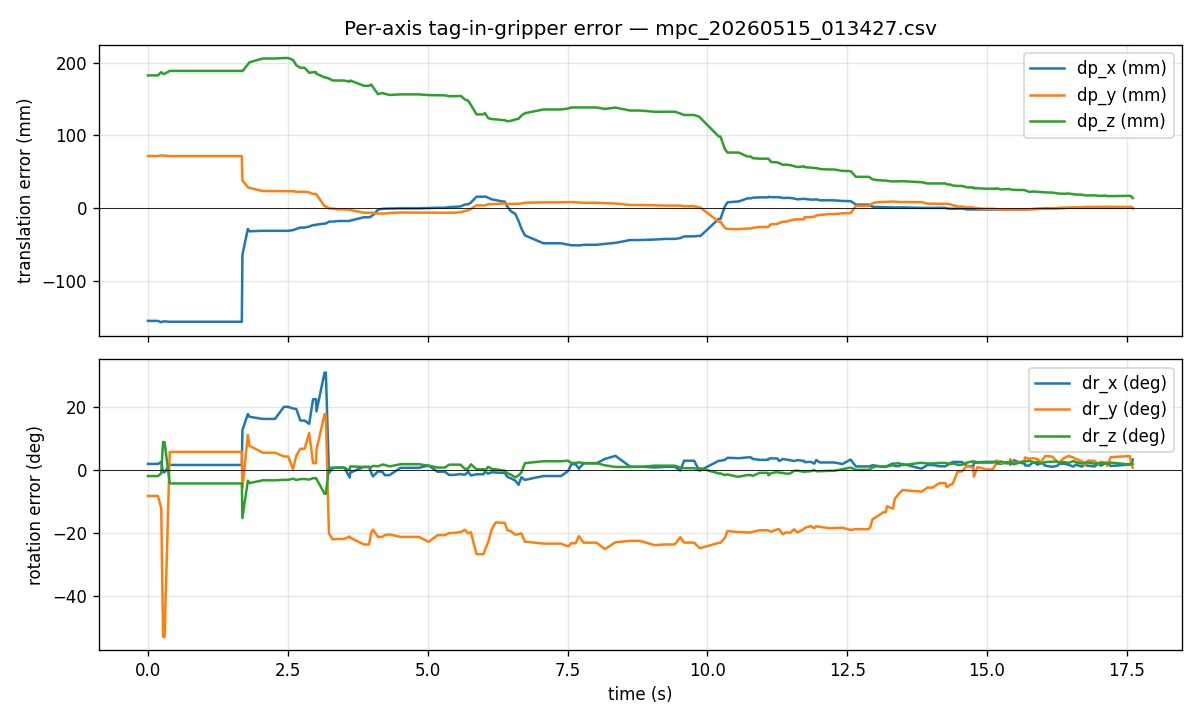
\includegraphics[width=\columnwidth]{mpc_per_axis.jpeg}
\caption{Error tag-en-gripper desglosado por eje. Arriba: componentes
de traslaci\'on $\Delta p_x, \Delta p_y, \Delta p_z$ en el marco
\texttt{gripper}. Abajo: componentes del error rotacional en
representaci\'on eje--\'angulo $\Delta r_x, \Delta r_y, \Delta r_z$
en grados.}
\label{fig:mpc-per-axis}
\end{figure}

La Fig.~\ref{fig:mpc-per-axis} permite ver la composici\'on interna
del error que la Fig.~\ref{fig:mpc-convergence} resume en una sola
norma. La componente $\Delta p_z$ (verde, eje \'optico del gripper)
es la dominante al inicio --- $\sim$\SI{200}{\milli\meter} --- y la
\'ultima en cancelarse, lo cual es esperable: representa la distancia
remanente a la botella, y solo se reduce conforme el brazo se acerca
en profundidad. Las componentes $\Delta p_x$ y $\Delta p_y$ caen mucho
m\'as r\'apido (en los primeros $\sim$\SI{5}{\second}), conforme el
MPC lateraliza el gripper para alinearlo. En el panel inferior, la
componente $\Delta r_y$ es la que m\'as tarde se corrige, lo cual
explica por qu\'e $\lVert\Delta\mathbf{r}\rVert$ se mantiene
estancada en torno a \SI{20}{\degree} hasta que esta componente
finalmente se anula cerca de $t\!\approx\!\SI{14}{\second}$.

\subsubsection{Twist comandado y restricciones de caja}

\begin{figure}[!t]
\centering
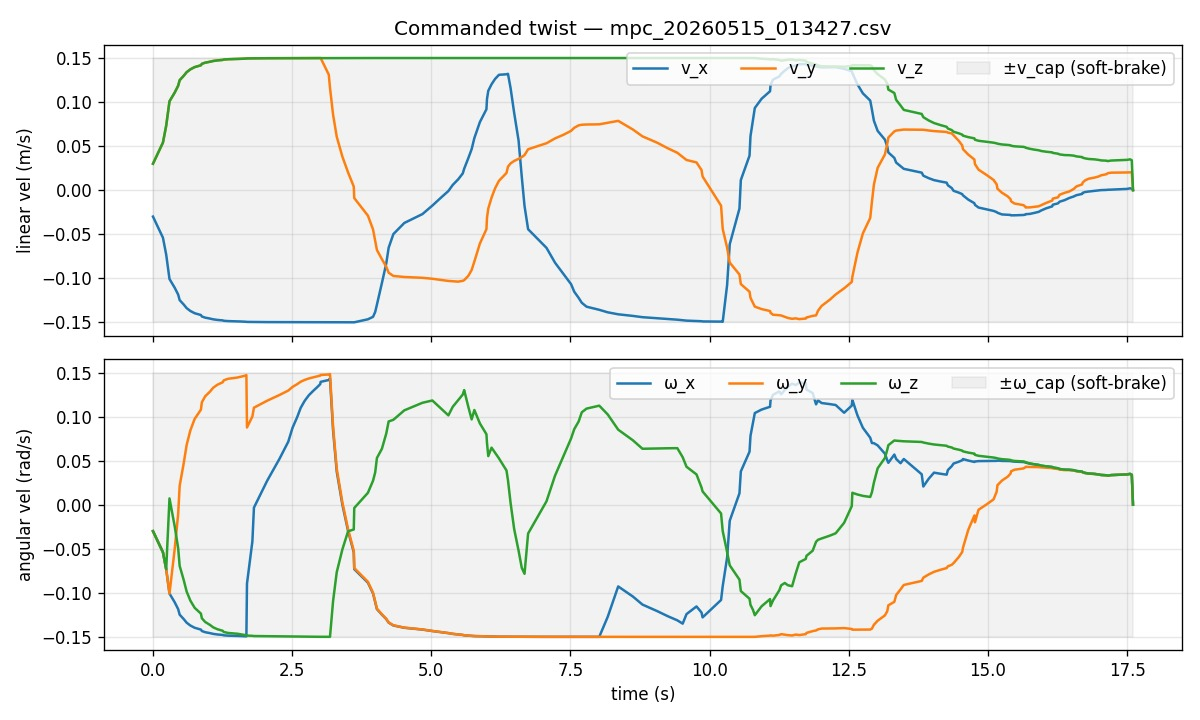
\includegraphics[width=\columnwidth]{mpc_commanded_twist.jpeg}
\caption{Twist Cartesiano comandado por el MPC y publicado a
\texttt{/servo\_node/delta\_twist\_cmds}. Arriba: velocidades lineales
$v_x, v_y, v_z$ en m/s; abajo: velocidades angulares
$\omega_x, \omega_y, \omega_z$ en rad/s. La banda gris representa los
l\'imites de caja $\pm v_\text{max}$ y $\pm\omega_\text{max}$
(\emph{soft-brake}) impuestos como restricciones del MPC.}
\label{fig:mpc-twist}
\end{figure}

La Fig.~\ref{fig:mpc-twist} muestra que el MPC opera la mayor parte
del tiempo en saturaci\'on positiva o negativa contra los l\'imites
de caja $v_\text{max}=\SI{0.15}{\meter\per\second}$ y
$\omega_\text{max}=\SI{0.15}{\radian\per\second}$, lo cual es el
comportamiento \'optimo esperado para un controlador con costo
cuadr\'atico y restricciones de caja: mientras el error es grande,
el solver elige el m\'aximo control admisible en la direcci\'on que
m\'as reduce el costo. Hacia el final de la corrida
($t\!>\!\SI{13}{\second}$) las velocidades empiezan a despegarse de
los l\'imites a medida que el costo de control $R$ domina sobre el
costo de estado $Q$ a errores peque\~nos, produciendo una desaceleraci\'on
suave que evita sobreimpulso al cierre.

\subsubsection{Suavizado EMA del comando}

\begin{figure}[!t]
\centering
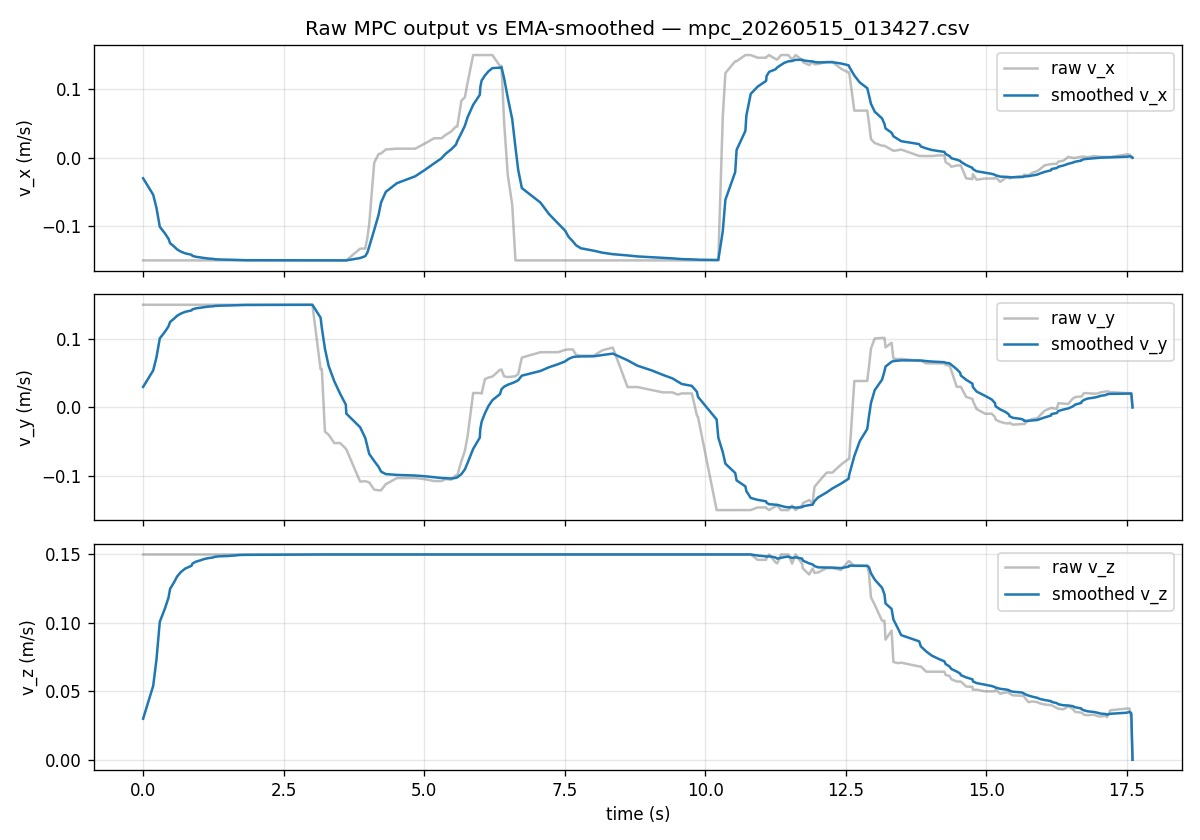
\includegraphics[width=\columnwidth]{mpc_raw_vs_smoothed.jpeg}
\caption{Salida cruda del MPC (gris) frente a la versi\'on suavizada
con un filtro exponencial m\'ovil (EMA, azul) que es la realmente
publicada al \texttt{servo\_node}. Se grafican las tres componentes
lineales $v_x, v_y, v_z$.}
\label{fig:mpc-smoothed}
\end{figure}

Como se observa en la Fig.~\ref{fig:mpc-smoothed}, la salida cruda
del solver presenta saltos abruptos cada vez que el modelo
linealizado cambia de signo o el AprilTag publica una nueva pose con
un peque\~no jitter. Estos saltos, aplicados directamente, generan
sacudidas en la articulaci\'on. Por ello el comando se filtra con
una EMA de constante de tiempo corta antes de ser publicado: la
curva azul reproduce el contenido de baja frecuencia de la se\~nal
gris pero elimina los escalones, manteniendo la latencia perceptible
por debajo de un ciclo de control y resultando en una trayectoria
articular notablemente m\'as fluida.

\subsection{Observaciones cualitativas}

\begin{itemize}
  \item La calibraci\'on \emph{hand--eye} fue el bloqueador
        principal en el desarrollo: con un mal \texttt{gripper}$\rightarrow$%
        \texttt{zed}, el MPC convergi\'a a poses sesgadas. Tras
        forzar variedad rotacional en las capturas, el RMS residual
        baj\'o a niveles aceptables y la convergencia del MPC se
        volvi\'o repetible.
  \item El cambio de FAR a NEAR durante la aproximaci\'on result\'o
        cr\'itico: un \'unico tag de un solo tama\'no o bien obliga a
        la c\'amara a ver bien desde lejos (sacrificando precisi\'on
        cerca) o bien deja al sistema sin se\~nal v\'alida durante
        gran parte del recorrido.
  \item La separaci\'on estricta entre etapas de MoveIt y de Servo,
        con pausas de asentamiento y reclamo expl\'icito del
        controlador, fue indispensable: la integraci\'on inicial
        sufri\'o fallos silenciosos que desaparecieron al imponer
        este orden.
\end{itemize}

% =====================================================================
\section{Conclusiones y trabajo futuro}
% =====================================================================

Se demostr\'o que un brazo xArm6 con un efector personalizado y dos
c\'amaras ZED puede ejecutar de forma aut\'onoma una tarea de
manipulaci\'on no trivial --- destapar una botella con un descorchador
de pared --- combinando servovisi\'on basada en MPC para el agarre y
alineaci\'on en espacio de imagen para la aproximaci\'on al mecanismo
de destape. La modularizaci\'on del pipeline en siete etapas
independientes facilit\'o el desarrollo incremental y el debugging:
cada subproceso puede ejecutarse y validarse de manera aislada.

\subsection*{Trabajo futuro}
\begin{itemize}
  \item Sustituir los AprilTags del descorchador por un detector
        geom\'etrico (Hough circles o segmentaci\'on por color) que
        no requiera modificar f\'isicamente la pared.
  \item Sustituir el cierre digital del gripper por una se\~nal de
        fuerza para confirmar agarre exitoso.
  \item Hacer adaptativos los pesos $Q$, $R$ del MPC en funci\'on de
        la distancia residual.
  \item A\~nadir tolerancia a botellas de diferentes tama\~nos
        re-aprendiendo \texttt{goal\_pose.yaml} en l\'inea.
\end{itemize}

% =====================================================================
\section*{Disponibilidad del c\'odigo y videos}

El c\'odigo, los lanzadores, las plantillas de AprilTag y los archivos
YAML de configuraci\'on se encuentran en el directorio
\texttt{Control\_Module/Visual\_Servoing\_Project/} del repositorio
del equipo:
\begin{center}
\url{https://github.com/GerardoFJ/TE3002B.102_Team2.git}
\end{center}

Los videos de demostraci\'on del sistema completo y de cada etapa del
pipeline est\'an disponibles en la siguiente carpeta de Google Drive:
\begin{center}
\url{https://drive.google.com/drive/folders/1zsFjLVak0Y8x4cpHOYnOJJxl5vdegP-K}
\end{center}

El stack base \emph{home2} se reutiliza desde el repositorio p\'ublico
de RoBorregos~\cite{roborregos-home2}:
\begin{center}
\url{https://github.com/RoBorregos/home2.git}
\end{center}

% =====================================================================
\begin{thebibliography}{9}

\bibitem{roborregos-home2}
RoBorregos, \emph{home2 -- stack de manipulaci\'on y navegaci\'on para
robot de servicio dom\'estico}, Tecnol\'ogico de Monterrey.
[Online]. Disponible en:
\url{https://github.com/RoBorregos/home2.git}

\bibitem{moveit-servo}
H. Bruyninckx \emph{et al.}, ``MoveIt Servo: real-time arm servoing in
ROS\,2,'' documentaci\'on oficial de MoveIt2, 2023.

\bibitem{apriltag}
E. Olson, ``AprilTag: A robust and flexible visual fiducial system,''
\emph{Proc.\ IEEE Int.\ Conf.\ Robotics and Automation}, 2011,
pp.~3400--3407.

\bibitem{tsai-handeye}
R.~Y. Tsai and R.~K. Lenz, ``A new technique for fully autonomous and
efficient 3D robotics hand/eye calibration,''
\emph{IEEE Trans.\ Robotics and Automation}, vol.~5, no.~3,
pp.~345--358, 1989.

\bibitem{mayne-mpc}
D.~Q. Mayne, J.~B. Rawlings, C.~V. Rao, and P.~O.~M. Scokaert,
``Constrained model predictive control: Stability and optimality,''
\emph{Automatica}, vol.~36, no.~6, pp.~789--814, 2000.

\end{thebibliography}

\end{document}
